\documentclass[12pt]{article}
\usepackage[margin=1in]{geometry}
\usepackage{amsmath,amssymb,mathtools}
\usepackage{enumitem}
\usepackage{bm}
\usepackage{hyperref}
\usepackage{fancyhdr}
\usepackage{draftwatermark}
\usepackage{xcolor}
\usepackage{pgfplots}
\usepackage{titlesec}
\pgfplotsset{compat=newest}

%------------- TITLE AND METADATA -------------
\newcommand{\CourseCode}{HE2001 }
\newcommand{\CourseName}{Microeconomics II}
\newcommand{\DocType}{Tutorial 8}

\title{
\CourseCode \CourseName \\[0.3em]
\large \DocType
}
\author{
  Academic Year 2025/2026, Semester 2 \\[0.25em]
  \textit{Quantitative Research Society @NTU}
}
\date{\today}

%------------- HEADER & FOOTER (for page 2 onward) -------------
\fancypagestyle{main}{
  \fancyhf{}
  \fancyhead[L]{\CourseCode \CourseName \ --\ \DocType}
  \fancyhead[R]{\href{https://qrsntu.org}{QRS@NTU}}
  \fancyfoot[C]{\thepage}
  \renewcommand{\headrulewidth}{0.4pt}
  \renewcommand{\footrulewidth}{0pt}
}

%------------- SIMPLE FOOTER (page 1 only) -------------
\fancypagestyle{plainfirst}{
  \fancyhf{}
  \renewcommand{\headrulewidth}{0pt}
  \renewcommand{\footrulewidth}{0pt}
  \fancyfoot[C]{\scriptsize\textcolor{gray}{\textit{For academic reference only. This document is provided for educational purposes and does not constitute an official question paper, answer key, or any formally authorised academic material. Its content is not guaranteed to be complete or accurate.}}}
}

%------------- WATERMARK -------------
\SetWatermarkText{Unofficial --- QRS@NTU --- qrsntu.org}
\SetWatermarkScale{1}
\SetWatermarkLightness{0.99}

%------------- SHORTCUTS -------------
\newcommand{\R}{\mathbb{R}}
\newcommand{\Rp}{\mathbb{R}_+}
\newcommand{\E}{\mathbb{E}}
\newcommand{\Var}{\mathrm{Var}}
\newcommand{\dotp}{\cdot}

%------------- STYLE REFINEMENTS -------------
\setlist[enumerate]{itemsep=0.32em, topsep=0.32em}
\setlist[itemize]{itemsep=0.22em, topsep=0.22em}

\titleformat{\subsubsection}[block]
{\normalfont\large\bfseries}
{}
{0pt}
{}

\titleformat{\paragraph}[block]
{\normalfont\normalsize\bfseries}
{}
{0pt}
{}

\titlespacing*{\paragraph}
{0pt}
{1.2ex}
{0.6ex}

%----------------------------------------
% Optional: tighter list defaults (feel free to adjust)
\setlist[enumerate]{itemsep=0.3em, topsep=0.3em}
\setlist[itemize]{itemsep=0.2em, topsep=0.2em}

\setcounter{secnumdepth}{-1} % Globally removes numbers from all sections
\setcounter{tocdepth}{3}     % Ensures \subsubsection level shows in TOC
\setlength{\headheight}{14.5pt}
\begin{document}

\maketitle
\thispagestyle{plainfirst}
\pagestyle{main}
\bigskip

%====================================================
% OVERVIEW
%====================================================
\begin{center}
  \rule{0.8\textwidth}{0.4pt}\\[4pt]
  \textbf{Overview}\\[2pt]
  \rule{0.8\textwidth}{0.4pt}
\end{center}

\noindent
This tutorial covers:
\begin{itemize}[leftmargin=*]
  \item per-unit subsidies, statutory incidence, and the role of supply and demand elasticities;
  \item ad-valorem taxation and welfare decomposition into consumer surplus, producer surplus, tax revenue, and deadweight welfare loss;
  \item horizontal summation of individual demand and supply curves in heterogeneous-consumer and multi-firm markets;
  \item equilibrium, consumer surplus, producer surplus, and deadweight loss under per-unit taxes;
  \item comparative tax incidence as the number of firms changes;
  \item past-year style applications involving quasilinear demand, kinked aggregate demand, and zero-trade equilibrium.
\end{itemize}

\bigskip

\newpage
\tableofcontents

%====================================================
% Question 1: Per-Unit Subsidies
%====================================================
\newpage
\section{Question 1: Per-Unit Subsidies}

\subsection{Problem}
\noindent
Let us consider the case of a per unit subsidy.

Assuming that we have linear supply curves and demand curves. Illustrate using a diagram:

For a) and b), indicate in the diagram(s) consumer surplus, producer surplus and amount of deadweight welfare loss.
\begin{enumerate}[label=(\alph*), leftmargin=*]
  \item The effects of a per unit subsidy of \(s\) on producers.
  \item The effects of a per unit subsidy of \(s\) on consumers.
  \item How do you think the elasticity of supply and demand will affect the incidence of benefits of a per unit subsidy on producers?
\end{enumerate}
\newpage
\subsection{Solution}

\begin{enumerate}[label=(\alph*)]
    \item If the subsidy is paid to producers, then for each unit sold producers receive the buyers' price plus the subsidy. If \(P_b\) denotes the price paid by buyers and \(P_s\) denotes the price received by sellers net of the subsidy, then
\[
P_s=P_b+s.
\]

\begin{center}
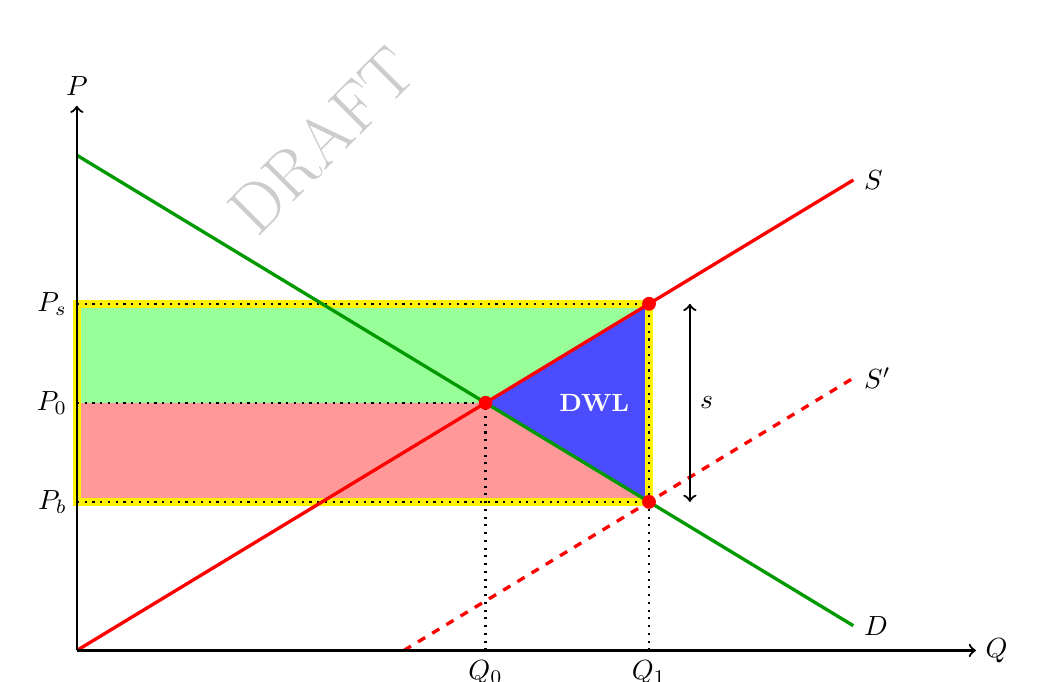
\begin{tikzpicture}

\begin{axis}[
    width=13cm,
    height=8.5cm,
    xmin=0,xmax=11,
    ymin=0,ymax=11,
    axis lines=left,
    axis line style={->, thick},
    axis on top=true,
    xlabel={$Q$},
    ylabel={$P$},
    xlabel style={at={(1,0)}, anchor=west},
    ylabel style={at={(0,1)}, anchor=south, rotate=-90},
    xtick=\empty,
    ytick=\empty,
    clip=false
]

\fill[red!40] (0, 3) -- (0, 5) -- (5, 5) -- (7, 3) -- cycle;
\fill[green!40] (0, 5) -- (0, 7) -- (7, 7) -- (5, 5) -- cycle;
\fill[blue!70] (5, 5) -- (7, 7) -- (7, 3) -- cycle;
\draw[yellow, line width=3pt] (0, 3) rectangle (7, 7);
\draw[thick, dotted] (0, 7) -- (7, 7);
\draw[thick, dotted] (0, 5) -- (5, 5);
\draw[thick, dotted] (0, 3) -- (7, 3);
\draw[thick, dotted] (5, 0) -- (5, 5);
\draw[thick, dotted] (7, 0) -- (7, 7);
\addplot[green!60!black, very thick, domain=0:9.5] {10-x} node[right, text=black] {$D$};
\addplot[red, very thick, domain=0:9.5] {x} node[right, text=black] {$S$};
\addplot[red, very thick, dashed, domain=4:9.5] {x-4} node[right, text=black] {$S'$};
\fill[red] (5,5) circle (2.5pt);
\fill[red] (7,7) circle (2.5pt);
\fill[red] (7,3) circle (2.5pt);
\node[left] at (0, 7) {$P_s$};
\node[left] at (0, 5) {$P_0$};
\node[left] at (0, 3) {$P_b$};
\node[below] at (5, 0) {$Q_0$};
\node[below] at (7, 0) {$Q_1$};
\node[text=white, font=\small\bfseries] at (6.33, 5) {DWL};
\draw[<->, thick] (7.5, 3) -- (7.5, 7) node[midway, right] {$s$};
\end{axis}
\end{tikzpicture}
\end{center}

The economic effects are:
\[
\boxed{\,Q \text{ rises},\quad P_b \text{ falls},\quad P_s \text{ rises},\quad \text{and DWL appears due to overproduction.}\,}
\]

\newpage
    \item If the subsidy is paid to consumers, then consumers pay the market price to sellers but recover \(s\) per unit from the government. If \(P_s\) denotes the price received by sellers and \(P_b\) denotes the net price borne by buyers, then
\[
P_s=P_b+s.
\]

\begin{center}
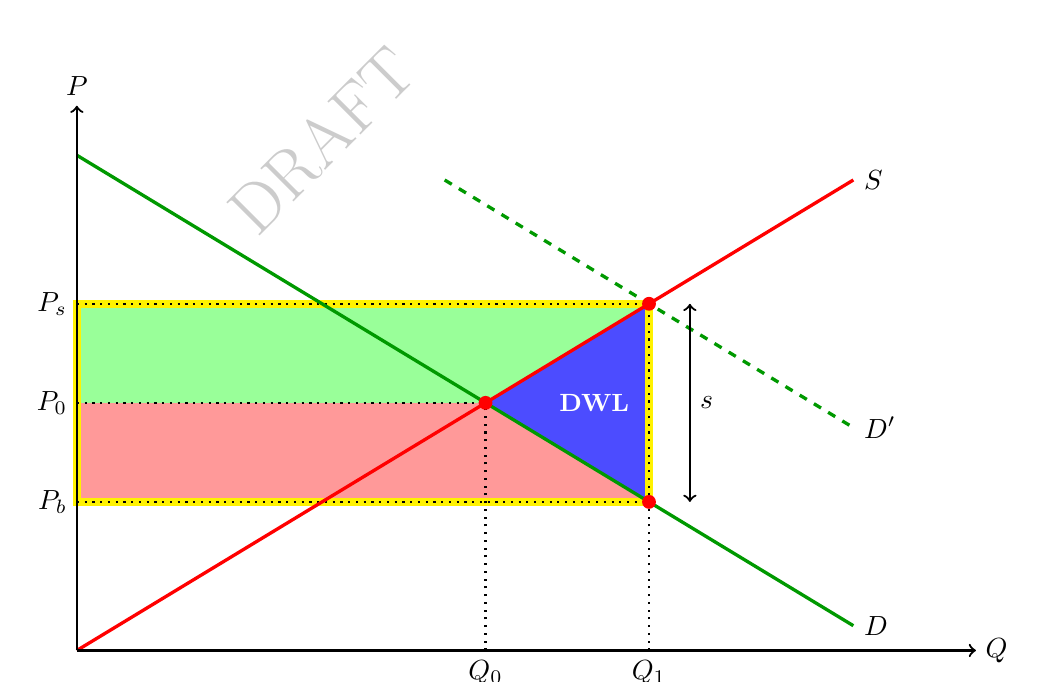
\begin{tikzpicture}
\begin{axis}[
    width=13cm,
    height=8.5cm,
    xmin=0,xmax=11,
    ymin=0,ymax=11,
    axis lines=left,
    axis line style={->, thick},
    axis on top=true,
    xlabel={$Q$},
    ylabel={$P$},
    xlabel style={at={(1,0)}, anchor=west},
    ylabel style={at={(0,1)}, anchor=south, rotate=-90},
    xtick=\empty,
    ytick=\empty,
    clip=false
]

\fill[red!40] (0, 3) -- (0, 5) -- (5, 5) -- (7, 3) -- cycle;
\fill[green!40] (0, 5) -- (0, 7) -- (7, 7) -- (5, 5) -- cycle;
\fill[blue!70] (5, 5) -- (7, 7) -- (7, 3) -- cycle;
\draw[yellow, line width=3pt] (0, 3) rectangle (7, 7);
\draw[thick, dotted] (0, 7) -- (7, 7);
\draw[thick, dotted] (0, 5) -- (5, 5);
\draw[thick, dotted] (0, 3) -- (7, 3);
\draw[thick, dotted] (5, 0) -- (5, 5);
\draw[thick, dotted] (7, 0) -- (7, 7);
\addplot[green!60!black, very thick, domain=0:9.5] {10-x} node[right, text=black] {$D$};
\addplot[green!60!black, very thick, dashed, domain=4.5:9.5] {14-x} node[right, text=black] {$D'$};
\addplot[red, very thick, domain=0:9.5] {x} node[right, text=black] {$S$};
\fill[red] (5,5) circle (2.5pt);
\fill[red] (7,7) circle (2.5pt);
\fill[red] (7,3) circle (2.5pt);
\node[left] at (0, 7) {$P_s$};
\node[left] at (0, 5) {$P_0$};
\node[left] at (0, 3) {$P_b$};
\node[below] at (5, 0) {$Q_0$};
\node[below] at (7, 0) {$Q_1$};
\node[text=white, font=\small\bfseries] at (6.33, 5) {DWL};
\draw[<->, thick] (7.5, 3) -- (7.5, 7) node[midway, right] {$s$};
\end{axis}
\end{tikzpicture}
\end{center}

Thus
\begin{center}
\fbox{\parbox{0.9\linewidth}{\centering
$Q$ rises, $P_b$ falls, $P_s$ rises, and deadweight loss appears due to overconsumption or overproduction.
}}
\end{center}

    \item The side of the market that is relatively less elastic captures more of the benefit from a subsidy. Therefore producers receive a larger share of the subsidy when:
    \begin{itemize}[leftmargin=*]
        \item supply is relatively more inelastic; and/or
        \item demand is relatively more elastic.
    \end{itemize}
    The intuition is standard. If producers are not very responsive to price, quantity supplied changes only a little, so more of the subsidy shows up as a higher price received by producers rather than as a lower price paid by consumers. If consumers are very price-sensitive, buyers' prices do not need to fall much to generate the additional quantity, so more of the subsidy remains with producers.

    Hence
    \begin{center}
    \fbox{\parbox{0.9\linewidth}{\centering
    Producers capture more of the subsidy when supply is more inelastic and demand is more elastic.
    }}
    \end{center}
\end{enumerate}


%====================================================
% SECTION 2
%====================================================
\newpage

%====================================================
% Question 2: Ad-Valorem Tax in the Car Market
%====================================================
\newpage
\section{Question 2: Ad-Valorem Tax in the Car Market}

\subsection{Problem}
\noindent
In the market for cars, the market demand curve is given by \(D(p) = 1200 - 100P\) while market supply curve is given by \(S(p) = 100p\).
\begin{enumerate}[label=(\alph*), leftmargin=*]
  \item Suppose that there is an ad-valorem (percentage) sales tax of 5 percent paid by consumers. I.e. \(P_B = 1.05P_S\), where \(P_B\) is the price paid by buyers and \(P_S\) is the price received by sellers. Solve for the equilibrium \(P_S\) and \(P_B\) and quantity in the market.
  \item Illustrate the effects of the ad-valorem tax above in a diagram, indicating the consumer surplus, producer surplus and deadweight welfare loss.
\end{enumerate}
\subsection{Solution}

\subsubsection{Method 1: Solve directly from the wedge condition}
\begin{enumerate}[label=(\alph*)]
    \item With the tax wedge,
    \[
    P_B=1.05P_S.
    \]
    Equilibrium requires demand at the buyers' price equals supply at the sellers' price:
    \[
    1200-100P_B=100P_S.
    \]
    Substitute \(P_B=1.05P_S\):
    \[
    1200-100(1.05P_S)=100P_S.
    \]
    So
    \[
    1200-105P_S=100P_S,
    \]
    hence
    \[
    1200=205P_S
    \quad\Longrightarrow\quad
    P_S=\frac{1200}{205}=\frac{240}{41}.
    \]
    Therefore
    \[
    P_B=1.05P_S=\frac{21}{20}\cdot \frac{240}{41}=\frac{252}{41}.
    \]
    The equilibrium quantity is
    \[
    Q=100P_S=100\cdot \frac{240}{41}=\frac{24000}{41}.
    \]
    Thus
    \[
    \boxed{\,P_S=\frac{240}{41},\qquad P_B=\frac{252}{41},\qquad Q=\frac{24000}{41}\,.}
    \]

    \item First compute the no-tax benchmark. Without tax,
    \[
    1200-100P=100P
    \quad\Longrightarrow\quad
    P_0=6,
    \qquad
    Q_0=600.
    \]
    In buyer-price space, the inverse demand and supply curves are
    \[
    P=12-\frac{Q}{100},
    \qquad
    P=\frac{Q}{100}.
    \]
    With the ad-valorem tax, buyers pay
    \[
    P_B=1.05P_S=1.05\cdot \frac{Q}{100},
    \]
    so the tax-distorted supply curve in buyer-price space is
    \[
    P_B=\frac{1.05Q}{100}.
    \]
    The post-tax equilibrium is
    \[
    \left(Q_t,P_B,P_S\right)=\left(\frac{24000}{41},\frac{252}{41},\frac{240}{41}\right).
    \]


\begin{center}
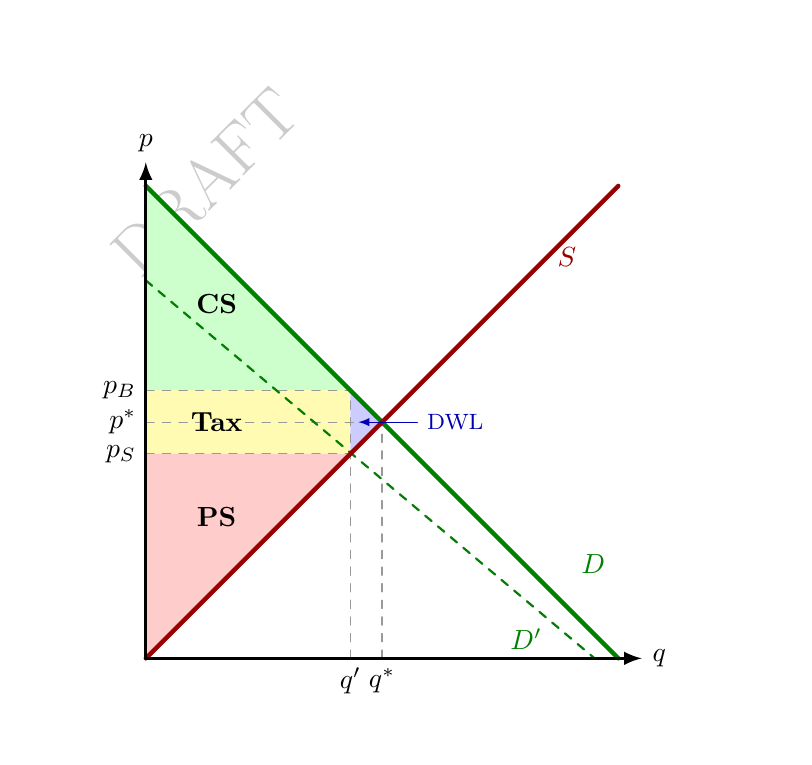
\begin{tikzpicture}[
    scale=3, % Increased scale for a better zoomed-in view
    >=latex,
    thick,
    line cap=round,
    label style/.style={font=\small}
]

% --- 1. SETTINGS & COLORS ---
\colorlet{cs_color}{green!20}
\colorlet{tr_color}{yellow!30}
\colorlet{ps_color}{red!20}
\colorlet{dwl_color}{blue!20}

% --- 2. CLIP COMMAND FOR ZOOM ---
% This restricts the drawing to our zoomed-in bounding box
\clip (3.0, 4.0) rectangle (6.2, 7.0);

% --- 3. SHADING (Drawn first so lines sit on top) ---
% Consumer Surplus
\fill[cs_color] (3.5, 5.634) -- (4.366, 5.634) -- (3.5, 6.5) -- cycle;
% Tax Revenue
\fill[tr_color] (3.5, 5.366) -- (4.366, 5.366) -- (4.366, 5.634) -- (3.5, 5.634) -- cycle;
% Producer Surplus
\fill[ps_color] (3.5, 4.5) -- (4.366, 5.366) -- (3.5, 5.366) -- cycle;
% Deadweight Loss
\fill[dwl_color] (4.366, 5.634) -- (4.5, 5.5) -- (4.366, 5.366) -- cycle;

% --- 4. PROJECTIONS ---
% Adjusted to start from the new localized axes origin (3.5, 4.5)
\draw[dashed, gray!80, thin] (3.5, 5.634) node[left, black] {$p_B$} -- (4.366, 5.634);
\draw[dashed, gray!80, thin] (3.5, 5.5) node[left, black] {$p^*$} -- (4.5, 5.5);
\draw[dashed, gray!80, thin] (3.5, 5.366) node[left, black] {$p_S$} -- (4.366, 5.366);
\draw[dashed, gray!80, thin] (4.366, 4.5) node[below, black] {$q'$} -- (4.366, 5.634);
\draw[dashed, gray!80, thin] (4.5, 4.5) node[below, black] {$q^*$} -- (4.5, 5.5);

% --- 5. CURVES ---
% Demand (D)
\draw[ultra thick, green!50!black] (3.5, 6.5) -- (5.5, 4.5);
\node[right, green!50!black] at (5.3, 4.9) {$D$};

% Shifted Demand (D')
\draw[thick, green!50!black, dashed] (3.5, 6.1) -- (5.4, 4.5);
\node[right, green!50!black] at (5, 4.58) {$D'$};

% Supply (S)
\draw[ultra thick, red!60!black] (3.5, 4.5) -- (5.5, 6.5);
\node[right, red!60!black] at (5.2, 6.2) {$S$};

% --- 6. LOCALIZED AXES ---
% Drawn inside the zoomed view
\draw[->, line width=1.2pt] (3.5, 4.5) -- (5.6, 4.5) node[right] {$q$};
\draw[->, line width=1.2pt] (3.5, 4.5) -- (3.5, 6.6) node[above] {$p$};

% --- 7. LABELS ---
% Relocated to fit nicely in the new frame
\node at (3.8, 6.0) {\textbf{CS}};
\node at (3.8, 5.5) {\textbf{Tax}};
\node at (3.8, 5.1) {\textbf{PS}};

% DWL Label with a pointer for maximum clarity in the tight space
\draw[<-, blue!70!black, thin] (4.4, 5.5) -- (4.65, 5.5) node[right] {\footnotesize DWL};

\end{tikzpicture}
\end{center}

\end{enumerate}

The corresponding exact welfare areas are:
\[
CS_t=\frac{1}{2}\cdot \frac{24000}{41}\left(12-\frac{252}{41}\right)
=\frac{2880000}{1681},
\]
\[
PS_t=\frac{1}{2}\cdot \frac{24000}{41}\cdot \frac{240}{41}
=\frac{2880000}{1681},
\]
\[
\text{Tax revenue}=(P_B-P_S)Q_t
=\left(\frac{12}{41}\right)\left(\frac{24000}{41}\right)
=\frac{288000}{1681},
\]
\[
DWL=\frac{1}{2}(Q_0-Q_t)(P_B-P_S)
=\frac{1}{2}\left(600-\frac{24000}{41}\right)\left(\frac{12}{41}\right)
=\frac{3600}{1681}.
\]
Hence
\[
\boxed{\,CS_t=\frac{2880000}{1681},\quad PS_t=\frac{2880000}{1681},\quad DWL=\frac{3600}{1681}\,.}
\]


\subsubsection{Method 2: Rewrite demand in terms of the sellers' price}
\begin{enumerate}[label=(\alph*)]
    \item Demand as a function of the sellers' price is
\[
Q_D=1200-100P_B
=1200-100(1.05P_S)
=1200-105P_S.
\]
Supply is
\[
Q_S=100P_S.
\]
Equating them,
\[
1200-105P_S=100P_S
\quad\Longrightarrow\quad
205P_S=1200
\quad\Longrightarrow\quad
P_S=\frac{240}{41}.
\]
Then
\[
P_B=\frac{21}{20}P_S=\frac{252}{41},
\qquad
Q=100P_S=\frac{24000}{41}.
\]
Hence
\[
\boxed{\,P_S=\frac{240}{41},\qquad P_B=\frac{252}{41},\qquad Q=\frac{24000}{41}\,.}
\]

\newpage


    \item Total-surplus comparison
Before tax,
\[
P_0=6,\qquad Q_0=600.
\]
Thus
\[
CS_0=\frac{1}{2}\cdot 600\cdot (12-6)=1800,
\qquad
PS_0=\frac{1}{2}\cdot 600\cdot 6=1800.
\]
So total surplus before tax is
\[
TS_0=3600.
\]
After tax,
\[
TS_t=CS_t+PS_t+\text{Tax revenue}
=\frac{2880000}{1681}+\frac{2880000}{1681}+\frac{288000}{1681}
=\frac{6048000}{1681}.
\]
Therefore
\[
DWL=TS_0-TS_t
=3600-\frac{6048000}{1681}
=\frac{3600}{1681}.
\]
This matches the triangle calculation in Method 1.

Thus
\[
\boxed{\,DWL=\frac{3600}{1681}\,.}
\]

\end{enumerate}

%====================================================
% SECTION 3
%====================================================
\newpage

%====================================================
% Question 3: Bubble Tea Market Aggregation
%====================================================
\newpage
\section{Question 3: Bubble Tea Market Aggregation}

\subsection{Problem}
\noindent
In the bubble tea market, there are 2 consumers with different preferences and 10 homogeneous firms. Consumer 1 has inverse demand function \(p = 20 - 4q_1\) while Consumer 2 has inverse demand function \(p = 15 - 2q_2\). Each of the firms has inverse supply function \(p = 5q_i\).
\begin{enumerate}[label=(\alph*), leftmargin=*]
  \item Derive the (aggregate) market supply curve and market demand curve.
  \item What is the equilibrium quantity and price in the market? Calculate the amount of producer and consumer surplus in the market.
  \item Suppose there is a per-unit tax on firms of \$0.5. What is the deadweight welfare loss from the tax?
\end{enumerate}

\newpage
\subsection{Solution}

\subsubsection{Method 1: Horizontal summation in direct-demand form}
\begin{enumerate}[label=(\alph*)]
    \item Consumer 1's inverse demand is
\[
p=20-4q_1
\quad\Longrightarrow\quad
q_1=\frac{20-p}{4}
\]
for \(0\le p\le 20\), and \(q_1=0\) for \(p>20\).

Consumer 2's inverse demand is
\[
p=15-2q_2
\quad\Longrightarrow\quad
q_2=\frac{15-p}{2}
\]
for \(0\le p\le 15\), and \(q_2=0\) for \(p>15\).

Hence the market demand is obtained by horizontal summation:
\[
Q_D(p)=q_1(p)+q_2(p).
\]
Therefore
\[
Q_D(p)=
\begin{cases}
\displaystyle \frac{20-p}{4}+\frac{15-p}{2}, & 0\le p\le 15,\\[0.9em]
\displaystyle \frac{20-p}{4}, & 15<p\le 20,\\[0.7em]
0, & p>20.
\end{cases}
\]
Simplifying the first branch,
\[
Q_D(p)=
\begin{cases}
\displaystyle \frac{50-3p}{4}, & 0\le p\le 15,\\[0.8em]
\displaystyle \frac{20-p}{4}, & 15<p\le 20,\\[0.7em]
0, & p>20.
\end{cases}
\]

Each firm's inverse supply is
\[
p=5q_i
\quad\Longrightarrow\quad
q_i=\frac{p}{5}.
\]
With 10 identical firms,
\[
Q_S(p)=10\cdot \frac{p}{5}=2p.
\]

Hence
\[
\boxed{\,
Q_D(p)=
\begin{cases}
\dfrac{50-3p}{4}, & 0\le p\le 15,\\[0.8em]
\dfrac{20-p}{4}, & 15<p\le 20,\\[0.7em]
0, & p>20,
\end{cases}
\qquad
Q_S(p)=2p.
\,}
\]


    \item Solve equilibrium in direct-demand form and sum surpluses by agent
Because the equilibrium price will turn out to be below \(15\), both consumers are active and the relevant demand branch is
\[
Q_D(p)=\frac{50-3p}{4}.
\]
Equate this with market supply:
\[
\frac{50-3p}{4}=2p.
\]
Thus
\[
50-3p=8p
\quad\Longrightarrow\quad
11p=50
\quad\Longrightarrow\quad
p^*=\frac{50}{11}.
\]
Then
\[
Q^*=2p^*=2\cdot \frac{50}{11}=\frac{100}{11}.
\]
So the equilibrium is
\[
\boxed{\,p^*=\frac{50}{11},\qquad Q^*=\frac{100}{11}\,.}
\]

Now compute each consumer's demand at the equilibrium price.

For Consumer 1,
\[
q_1^*=\frac{20-p^*}{4}
=\frac{20-\frac{50}{11}}{4}
=\frac{85}{22}.
\]
For Consumer 2,
\[
q_2^*=\frac{15-p^*}{2}
=\frac{15-\frac{50}{11}}{2}
=\frac{115}{22}.
\]
Their consumer surpluses are:
\[
CS_1=\frac{1}{2}q_1^*(20-p^*)
=\frac{1}{2}\cdot \frac{85}{22}\cdot \frac{170}{11}
=\frac{7225}{242},
\]
\[
CS_2=\frac{1}{2}q_2^*(15-p^*)
=\frac{1}{2}\cdot \frac{115}{22}\cdot \frac{115}{11}
=\frac{13225}{484}.
\]
So total consumer surplus is
\[
CS=CS_1+CS_2=\frac{7225}{242}+\frac{13225}{484}
=\frac{27675}{484}.
\]

Each firm's output is
\[
q_i^*=\frac{p^*}{5}=\frac{10}{11}.
\]
Each firm has a linear inverse supply through the origin, so producer surplus per firm is
\[
PS_i=\frac{1}{2}q_i^*p^*
=\frac{1}{2}\cdot \frac{10}{11}\cdot \frac{50}{11}
=\frac{250}{121}.
\]
With 10 firms,
\[
PS=10PS_i=\frac{2500}{121}.
\]

Therefore
\[
\boxed{\,CS=\frac{27675}{484},\qquad PS=\frac{2500}{121}\,.}
\]


    \item Wedge-and-triangle calculation
A per-unit tax of \(t=0.5\) on firms creates the wedge
\[
p_b=p_s+t=p_s+\frac{1}{2}.
\]
Each firm's supply becomes
\[
q_i=\frac{p_s}{5}=\frac{p_b-\frac{1}{2}}{5},
\]
so aggregate supply in terms of the buyers' price is
\[
Q_S^t(p_b)=10\cdot \frac{p_b-\frac{1}{2}}{5}=2p_b-1.
\]
The relevant demand branch remains
\[
Q_D(p_b)=\frac{50-3p_b}{4}.
\]
Equating demand and taxed supply,
\[
\frac{50-3p_b}{4}=2p_b-1.
\]
Therefore
\[
50-3p_b=8p_b-4
\quad\Longrightarrow\quad
54=11p_b
\quad\Longrightarrow\quad
p_b=\frac{54}{11}.
\]
Hence
\[
Q_t=2p_b-1=\frac{108}{11}-1=\frac{97}{11}.
\]
Without tax,
\[
Q_0=\frac{100}{11}.
\]
So the fall in quantity is
\[
Q_0-Q_t=\frac{100}{11}-\frac{97}{11}=\frac{3}{11}.
\]
The deadweight loss is the triangle
\[
DWL=\frac{1}{2}\cdot t \cdot (Q_0-Q_t)
=\frac{1}{2}\cdot \frac{1}{2}\cdot \frac{3}{11}
=\frac{3}{44}.
\]
Thus
\[
\boxed{\,DWL=\frac{3}{44}\,.}
\]
\end{enumerate}

\newpage
\subsubsection{Method 2: Inverse-curve representation}
\begin{enumerate}[label=(\alph*)]
    \item For the demand side, note the kink occurs where Consumer 2 just drops out, namely at \(p=15\). At that price Consumer 1 still demands
\[
q_1=\frac{20-15}{4}=\frac{5}{4},
\]
so the market-demand kink is at
\[
\left(Q,p\right)=\left(\frac{5}{4},15\right).
\]
Thus the inverse market demand is
\[
p=
\begin{cases}
20-4Q, & 0\le Q\le \frac{5}{4},\\[0.7em]
\displaystyle \frac{50-4Q}{3}, & \frac{5}{4}\le Q\le \frac{25}{2}.
\end{cases}
\]
For supply, since \(Q_S=2p\), the inverse market supply is
\[
p=\frac{Q}{2}.
\]
Therefore
\[
\boxed{\,
p_D(Q)=
\begin{cases}
20-4Q, & 0\le Q\le \frac{5}{4},\\[0.7em]
\dfrac{50-4Q}{3}, & \frac{5}{4}\le Q\le \frac{25}{2},
\end{cases}
\qquad
p_S(Q)=\frac{Q}{2}.
\,}
\]

    \item Use inverse market curves and integrate
From Question 3.1, the inverse market demand is
\[
p_D(Q)=
\begin{cases}
20-4Q, & 0\le Q\le \frac{5}{4},\\[0.7em]
\dfrac{50-4Q}{3}, & \frac{5}{4}\le Q\le \frac{25}{2},
\end{cases}
\qquad
p_S(Q)=\frac{Q}{2}.
\]
Since \(Q^*=\frac{100}{11}>\frac{5}{4}\), the relevant demand branch at equilibrium is
\[
\frac{50-4Q}{3}=\frac{Q}{2}.
\]
Multiplying through by \(6\),
\[
100-8Q=3Q
\quad\Longrightarrow\quad
11Q=100
\quad\Longrightarrow\quad
Q^*=\frac{100}{11},
\]
and hence
\[
p^*=\frac{Q^*}{2}=\frac{50}{11}.
\]

Consumer surplus is the area under inverse demand above \(p^*\):
\begin{align*}
CS
&=\int_0^{5/4}(20-4Q)\,dQ
+\int_{5/4}^{100/11}\frac{50-4Q}{3}\,dQ
-\frac{50}{11}\cdot \frac{100}{11}\\
&=\frac{175}{8}+\frac{74175}{968}-\frac{5000}{121}
=\frac{27675}{484}.
\end{align*}
Producer surplus is the area above inverse supply and below \(p^*\):
\[
PS=\frac{1}{2}Q^*p^*
=\frac{1}{2}\cdot \frac{100}{11}\cdot \frac{50}{11}
=\frac{2500}{121}.
\]
Thus
\[
\boxed{\,p^*=\frac{50}{11},\qquad Q^*=\frac{100}{11},\qquad CS=\frac{27675}{484},\qquad PS=\frac{2500}{121}\,.}
\]


    \item Total-surplus comparison
From Question 3.2, pre-tax total surplus is
\[
TS_0=CS_0+PS_0=\frac{27675}{484}+\frac{2500}{121}=\frac{3425}{44}.
\]

Under the tax, we already found
\[
p_b=\frac{54}{11},\qquad Q_t=\frac{97}{11}.
\]
The price received by sellers is
\[
p_s=p_b-\frac{1}{2}=\frac{54}{11}-\frac{1}{2}=\frac{97}{22}.
\]
Consumer surplus is
\[
CS_t=\frac{26099}{484},
\]
producer surplus is
\[
PS_t=\frac{9409}{484},
\]
and tax revenue is
\[
TR=tQ_t=\frac{1}{2}\cdot \frac{97}{11}=\frac{97}{22}.
\]
Therefore
\[
TS_t=CS_t+PS_t+TR
=\frac{26099}{484}+\frac{9409}{484}+\frac{97}{22}
=\frac{1711}{22}.
\]
Hence
\[
DWL=TS_0-TS_t
=\frac{3425}{44}-\frac{1711}{22}
=\frac{3425-3422}{44}
=\frac{3}{44}.
\]
So
\[
\boxed{\,DWL=\frac{3}{44}\,.}
\]
\end{enumerate}

%====================================================
% SECTION 4
%====================================================
\newpage

%====================================================
% Question 4: Mala-Hotpot Excise Tax
%====================================================
\newpage
\section{Question 4: Mala-Hotpot Excise Tax}

\subsection{Problem}
\noindent
In the mala-hotpot market, market demand is given by \(D(P_b) = 1000 - 10P_b\).

The individual supply of each stall is given by \(S_i(P_s) = 10P_s - 10\). Suppose there are \(n\) identical stalls in the market. As the government thinks that mala-hotpot is unhealthy, it decides to implement a per-unit excise tax of \$2.
\begin{enumerate}[label=(\alph*), leftmargin=*]
  \item Solve for the equilibrium price and quantity in this market without any taxes (as a function of \(n\)).
  \item Solve for the equilibrium prices and quantity in this market with the per-unit tax (as a function of \(n\)).
  \item How does the incidence of tax on consumers change as the number of stalls \(n\) increases? Explain the intuition behind this.
\end{enumerate}
\subsection{Solution}

\subsubsection{Method 1: Aggregate supply then equate demand and supply}
\begin{enumerate}[label=(\alph*)]
    \item Without tax, buyers' and sellers' prices coincide:
\[
P_b=P_s=P.
\]
Each stall supplies
\[
q_i=10P-10.
\]
With \(n\) identical stalls, market supply is
\[
Q_S=n(10P-10)=10nP-10n.
\]
Market demand is
\[
Q_D=1000-10P.
\]
Equilibrium requires
\[
1000-10P=10nP-10n.
\]
So
\[
1000+10n=10P(n+1).
\]
Hence
\[
P^*=\frac{100+n}{n+1}.
\]
Substituting into demand,
\begin{align*}
Q^*
&=1000-10\left(\frac{100+n}{n+1}\right)\\
&=\frac{1000(n+1)-10(100+n)}{n+1}\\
&=\frac{1000n+1000-1000-10n}{n+1}\\
&=\frac{990n}{n+1}.
\end{align*}
Therefore
\[
\boxed{\,P^*=\frac{100+n}{n+1},\qquad Q^*=\frac{990n}{n+1}\,.}
\]


    \item Buyers' price, sellers' price, and the tax wedge
With a per-unit tax of \(2\),
\[
P_b=P_s+2.
\]
Market demand is
\[
Q_D=1000-10P_b,
\]
and market supply is
\[
Q_S=10nP_s-10n.
\]
Equilibrium requires
\[
1000-10(P_s+2)=10nP_s-10n.
\]
So
\[
980=10(n+1)P_s-10n,
\]
hence
\[
98=(n+1)P_s-n.
\]
Therefore
\[
P_s=\frac{98+n}{n+1}.
\]
Then
\[
P_b=P_s+2
=\frac{98+n}{n+1}+2
=\frac{100+3n}{n+1}.
\]
The equilibrium quantity is
\[
Q_t=10nP_s-10n
=10n\left(\frac{98+n}{n+1}-1\right)
=10n\left(\frac{97}{n+1}\right)
=\frac{970n}{n+1}.
\]
Hence
\[
\boxed{\,P_s=\frac{98+n}{n+1},\qquad P_b=\frac{100+3n}{n+1},\qquad Q_t=\frac{970n}{n+1}\,.}
\]


    \item Compare the pre-tax and post-tax prices
From Question 4.1,
\[
P^*=\frac{100+n}{n+1}.
\]
From Question 4.2,
\[
P_b=\frac{100+3n}{n+1},
\qquad
P_s=\frac{98+n}{n+1}.
\]
Hence the amount of the tax borne by consumers is
\[
P_b-P^*
=\frac{100+3n}{n+1}-\frac{100+n}{n+1}
=\frac{2n}{n+1}.
\]
The amount borne by producers is
\[
P^*-P_s
=\frac{100+n}{n+1}-\frac{98+n}{n+1}
=\frac{2}{n+1}.
\]
These add up to the full tax:
\[
\frac{2n}{n+1}+\frac{2}{n+1}=2.
\]
Therefore the consumer share of the tax is
\[
\frac{P_b-P^*}{2}=\frac{n}{n+1}.
\]
As \(n\) increases,
\[
\frac{n}{n+1}\uparrow 1.
\]
So consumers bear a larger and larger fraction of the tax, and in the limit they bear almost all of it.

Thus
\[
\boxed{\,\text{Consumer incidence rises with }n,\ \text{and tends to the full \$2 tax as }n\to\infty.\,}
\]
\end{enumerate}

\newpage
\subsubsection{Method 2: Inverse supply representation}
\begin{enumerate}[label=(\alph*)]
    \item Each stall's direct supply is
\[
q_i=10P_s-10
\quad\Longrightarrow\quad
P_s=1+\frac{q_i}{10}.
\]
With \(n\) identical stalls, if total output is \(Q\), symmetry implies each stall supplies \(q_i=Q/n\). Hence the inverse market supply is
\[
P=1+\frac{Q}{10n}.
\]
The inverse demand is
\[
P=100-\frac{Q}{10}.
\]
Equating inverse demand and inverse supply,
\[
100-\frac{Q}{10}=1+\frac{Q}{10n}.
\]
Therefore
\[
99=\frac{Q}{10}+\frac{Q}{10n}
=\frac{Q(n+1)}{10n}.
\]
So
\[
Q^*=\frac{990n}{n+1}.
\]
Then
\[
P^*=100-\frac{Q^*}{10}
=100-\frac{99n}{n+1}
=\frac{100+n}{n+1}.
\]
Thus
\[
\boxed{\,P^*=\frac{100+n}{n+1},\qquad Q^*=\frac{990n}{n+1}\,.}
\]


    \item Inverse supply shifted by the tax
Without tax, the inverse market supply is
\[
P_s=1+\frac{Q}{10n}.
\]
A tax of \(2\) raises the buyers' price needed to induce any given quantity by \(2\), so in buyers' price terms the taxed inverse supply is
\[
P_b=3+\frac{Q}{10n}.
\]
Inverse demand is
\[
P_b=100-\frac{Q}{10}.
\]
Equating them,
\[
100-\frac{Q}{10}=3+\frac{Q}{10n}.
\]
Thus
\[
97=\frac{Q}{10}+\frac{Q}{10n}
=\frac{Q(n+1)}{10n},
\]
so
\[
Q_t=\frac{970n}{n+1}.
\]
Then
\[
P_b=100-\frac{Q_t}{10}
=100-\frac{97n}{n+1}
=\frac{100+3n}{n+1},
\]
and
\[
P_s=P_b-2=\frac{98+n}{n+1}.
\]
Therefore
\[
\boxed{\,P_s=\frac{98+n}{n+1},\qquad P_b=\frac{100+3n}{n+1},\qquad Q_t=\frac{970n}{n+1}\,.}
\]


    \item Elasticity intuition via market supply
The aggregate supply curve is
\[
Q_S=10nP_s-10n.
\]
In inverse form,
\[
P_s=1+\frac{Q}{10n}.
\]
As \(n\) increases, the coefficient \(1/(10n)\) becomes smaller, so the inverse supply curve becomes flatter. Equivalently, aggregate supply becomes more elastic.

When supply is very elastic, firms are unwilling to absorb much of the tax through a lower net-of-tax price. Instead, most of the tax is passed on to consumers in the form of a higher buyers' price. That is exactly what the formula
\[
P_b-P^*=\frac{2n}{n+1}
\]
shows.

Hence
\[
\boxed{\,\text{More stalls } \Rightarrow \text{ more elastic market supply } \Rightarrow \text{ higher consumer tax incidence.}\,}
\]

%====================================================
% SECTION 5
%====================================================
\end{enumerate}

%====================================================
% Sample Question 1: Good X
%====================================================

\newpage
\section{Sample Question 1: Good X with Heterogeneous Consumers and Firms}

\subsection{Problem}

\noindent
In the market for good \(X\), which has a price of \(p\), there are 160 consumers with an identical income of \$100. There are two types of consumers, Type 1 and Type 2, each with different preferences.

\noindent
Type 1s have preferences
\[
U_1(x)=16x-4x^2+m,
\]
where \(x\) is the quantity of good \(x\) purchased and \(m\) is their leftover cash holdings. Type 2s have preferences
\[
U_2(x)=8x-8x^2+m.
\]

\bigskip
\noindent There are 80 consumers of Type 1 and 80 consumers of Type 2.

\begin{enumerate}[label=(\alph*)]
    \item Derive the individual demand curves for Type 1 and Type 2 consumers. \hfill \textbf{(6 marks)}
    \item Derive the aggregate demand curve for good \(X\). \hfill \textbf{(5 marks)}
\end{enumerate}


\bigskip
\noindent
In the market for good \(X\), there are also a total of \(n\) identical firms who are profit maximisers. Each of these firms has a cost function of$3x^2.$
\begin{enumerate}[label=(\alph*), start=3]
    \item Maximise the profits of each firm \((px-3x^2)\) to derive the individual supply curve. Subsequently derive the aggregate supply curve for good \(X\). \hfill \textbf{(5 marks)}
    \item How does the market’s elasticity of supply change with the number of firms in the market? Explain. \hfill \textbf{(4 marks)}
\end{enumerate}

\bigskip
\noindent
Suppose that \(n=72\), i.e. there are 72 firms in the market.

\begin{enumerate}[label=(\alph*), start=5]
    \item Draw out the aggregate demand and supply curves in the market, calculating and indicating the exact market equilibrium on your figure. \hfill \textbf{(7 marks)}
    \item What is the amount of consumer and producer surplus in the market? \hfill \textbf{(5 marks)}
\end{enumerate}

\noindent
Suppose that the government now imposes a per unit tax of \$6 on producers.

\begin{enumerate}[label=(\alph*), start=7]
    \item Illustrate in a diagram, as accurately as possible, the effect of the tax, indicating i) the deadweight welfare loss, and ii) the incidence of the tax burden on consumers and producers. \hfill \textbf{(8 marks)}
\end{enumerate}


\newpage
\subsection{Solution}

\subsubsection{Method 1: Direct optimisation, aggregation, and equilibrium solving}

\begin{enumerate}[label=(\alph*)]
    \item
    For Type 1, since leftover cash is
    \[
    m=100-px,
    \]
    utility becomes
    \[
    U_1(x)=16x-4x^2+100-px.
    \]
    Differentiate:
    \[
    \frac{dU_1}{dx}=16-8x-p.
    \]
    Setting the first-order condition equal to zero,
    \[
    16-8x-p=0
    \quad\Longrightarrow\quad
    x=\frac{16-p}{8}=2-\frac{p}{8}.
    \]
    Because
    \[
    \frac{d^2U_1}{dx^2}=-8<0,
    \]
    this is the maximiser whenever it is nonnegative. Hence
    \[
    x_1(p)=
    \begin{cases}
    2-\dfrac{p}{8}, & 0\le p\le 16,\\[0.6em]
    0, & p>16.
    \end{cases}
    \]

    For Type 2,
    \[
    U_2(x)=8x-8x^2+100-px.
    \]
    Differentiate:
    \[
    \frac{dU_2}{dx}=8-16x-p.
    \]
    Setting this equal to zero,
    \[
    8-16x-p=0
    \quad\Longrightarrow\quad
    x=\frac{8-p}{16}=\frac12-\frac{p}{16}.
    \]
    Since
    \[
    \frac{d^2U_2}{dx^2}=-16<0,
    \]
    this is the maximiser whenever nonnegative. Therefore
    \[
    x_2(p)=
    \begin{cases}
    \dfrac12-\dfrac{p}{16}, & 0\le p\le 8,\\[0.6em]
    0, & p>8.
    \end{cases}
    \]

    Thus
    \[
    \boxed{
    x_1(p)=
    \begin{cases}
    2-\dfrac{p}{8}, & 0\le p\le 16,\\[0.5em]
    0, & p>16,
    \end{cases}
    \qquad
    x_2(p)=
    \begin{cases}
    \dfrac12-\dfrac{p}{16}, & 0\le p\le 8,\\[0.5em]
    0, & p>8.
    \end{cases}}
    \]

    \item
    There are 80 consumers of each type, so aggregate demand is
    \[
    Q_D(p)=80x_1(p)+80x_2(p).
    \]

    For \(0\le p\le 8\), both types buy:
    \begin{align*}
    Q_D(p)
    &=80\left(2-\frac{p}{8}\right)+80\left(\frac12-\frac{p}{16}\right)\\
    &=160-10p+40-5p\\
    &=200-15p.
    \end{align*}

    For \(8<p\le 16\), only Type 1 buys:
    \[
    Q_D(p)=80\left(2-\frac{p}{8}\right)=160-10p.
    \]

    For \(p>16\), nobody buys:
    \[
    Q_D(p)=0.
    \]

    Hence
    \[
    \boxed{
    Q_D(p)=
    \begin{cases}
    200-15p, & 0\le p\le 8,\\[0.4em]
    160-10p, & 8<p\le 16,\\[0.4em]
    0, & p>16.
    \end{cases}}
    \]

    \item
    Each firm solves
    \[
    \max_{x\ge 0}\; \pi(x)=px-3x^2.
    \]
    Differentiate:
    \[
    \frac{d\pi}{dx}=p-6x.
    \]
    Setting this equal to zero,
    \[
    p-6x=0
    \quad\Longrightarrow\quad
    x=\frac{p}{6}.
    \]
    Since
    \[
    \frac{d^2\pi}{dx^2}=-6<0,
    \]
    this is the profit-maximising quantity. Therefore the individual supply curve is
    \[
    \boxed{x_s(p)=\frac{p}{6}.}
    \]

    With \(n\) identical firms, aggregate supply is
    \[
    Q_S(p)=n\frac{p}{6}.
    \]
    So
    \[
    \boxed{Q_S(p)=\frac{n}{6}p.}
    \]

    \item
    Since
    \[
    Q_S(p)=\frac{n}{6}p,
    \]
    we have
    \[
    \frac{dQ_S}{dp}=\frac{n}{6}.
    \]
    The price elasticity of supply is
    \[
    \varepsilon_S=\frac{dQ_S}{dp}\cdot \frac{p}{Q_S(p)}
    =\frac{n}{6}\cdot \frac{p}{(n/6)p}=1.
    \]
    Hence the market’s elasticity of supply does not change with the number of firms:
    \[
    \boxed{\varepsilon_S=1\text{ for all }p>0.}
    \]

    The number of firms changes the scale of market supply, but not its elasticity.

    \item
    Set \(n=72\). Then market supply is
    \[
    Q_S(p)=\frac{72}{6}p=12p.
    \]
    Since the equilibrium price will turn out to be below 8, the relevant demand branch is
    \[
    Q_D(p)=200-15p.
    \]
    Equating demand and supply,
    \[
    200-15p=12p.
    \]
    Hence
    \[
    27p=200
    \quad\Longrightarrow\quad
    p^*=\frac{200}{27}.
    \]
    Therefore
    \[
    Q^*=12p^*=\frac{800}{9}.
    \]

    Thus
    \[
    \boxed{p^*=\frac{200}{27},\qquad Q^*=\frac{800}{9}.}
    \]

    A suitable graph is:

    \begin{center}
    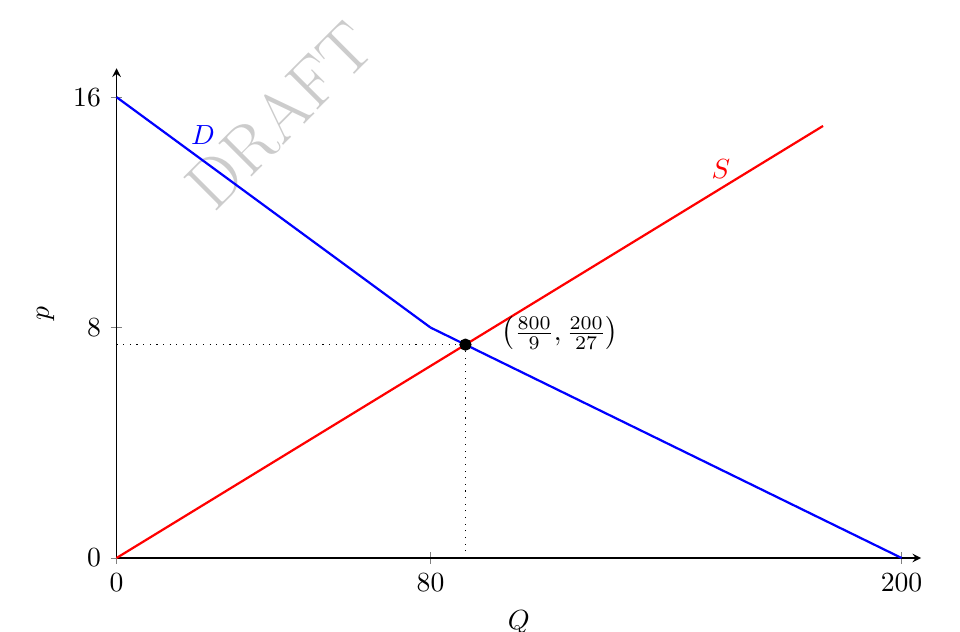
\begin{tikzpicture}
    \begin{axis}[
        width=11.8cm,
        height=7.8cm,
        xmin=0,xmax=205,
        ymin=0,ymax=17,
        axis lines=left,
        xlabel={$Q$},
        ylabel={$p$},
        xtick={0,80,200},
        xticklabels={$0$,$80$,$200$},
        ytick={0,8,16},
        yticklabels={$0$,$8$,$16$},
        clip=false
    ]
    \addplot[thick,blue] coordinates {(0,16) (80,8)};
    \addplot[thick,blue] coordinates {(80,8) (200,0)};
    \addplot[thick,red,domain=0:180,samples=2] {x/12};

    \addplot[dotted] coordinates {(88.8889,0) (88.8889,7.4074)};
    \addplot[dotted] coordinates {(0,7.4074) (88.8889,7.4074)};
    \addplot[only marks,mark=*,mark size=2pt] coordinates {(88.8889,7.4074)};

    \node[blue] at (axis cs:22,14.7) {$D$};
    \node[red] at (axis cs:154,13.5) {$S$};
    \node at (axis cs:113,7.8) {$\left(\frac{800}{9},\frac{200}{27}\right)$};
    \end{axis}
    \end{tikzpicture}
    \end{center}

    \item
    At the equilibrium price \(p^*=\frac{200}{27}\), Type 1 buys
    \[
    x_1^*=2-\frac{1}{8}\cdot \frac{200}{27}
    =2-\frac{25}{27}
    =\frac{29}{27},
    \]
    while Type 2 buys
    \[
    x_2^*=\frac12-\frac{1}{16}\cdot \frac{200}{27}
    =\frac12-\frac{25}{54}
    =\frac{1}{27}.
    \]

    Type 1 consumer surplus per consumer is
    \[
    CS_1^{\text{ind}}
    =\frac12\left(16-\frac{200}{27}\right)\frac{29}{27}
    =\frac{3364}{729}.
    \]
    Across 80 Type 1 consumers:
    \[
    CS_1=80\cdot \frac{3364}{729}=\frac{269120}{729}.
    \]

    Type 2 consumer surplus per consumer is
    \[
    CS_2^{\text{ind}}
    =\frac12\left(8-\frac{200}{27}\right)\frac{1}{27}
    =\frac{8}{729}.
    \]
    Across 80 Type 2 consumers:
    \[
    CS_2=80\cdot \frac{8}{729}=\frac{640}{729}.
    \]

    Therefore
    \[
    CS=CS_1+CS_2=\frac{269760}{729}=\frac{89920}{243}.
    \]
    So
    \[
    \boxed{CS=\frac{89920}{243}.}
    \]

    Producer surplus is
    \[
    PS=\frac12 p^*Q^*
    =\frac12\cdot \frac{200}{27}\cdot \frac{800}{9}
    =\frac{80000}{243}.
    \]
    Hence
    \[
    \boxed{PS=\frac{80000}{243}.}
    \]

    \item
    A per-unit tax of \(6\) on producers implies
    \[
    p_b=p_s+6.
    \]
    Since aggregate supply before tax is
    \[
    Q_S=12p_s,
    \]
    aggregate supply in terms of the buyers' price is
    \[
    Q_S^t(p_b)=12(p_b-6)=12p_b-72.
    \]
    After tax the buyers' price exceeds 8, so only Type 1 remains active. Hence the relevant demand branch is
    \[
    Q_D(p_b)=160-10p_b.
    \]
    Equating demand and taxed supply,
    \[
    160-10p_b=12p_b-72.
    \]
    Therefore
    \[
    232=22p_b
    \quad\Longrightarrow\quad
    p_b=\frac{116}{11}.
    \]
    The taxed quantity is
    \[
    Q_t=160-10p_b=\frac{600}{11},
    \]
    and the sellers' net price is
    \[
    p_s=p_b-6=\frac{50}{11}.
    \]

    Thus
    \[
    \boxed{p_b=\frac{116}{11},\qquad p_s=\frac{50}{11},\qquad Q_t=\frac{600}{11}.}
    \]

    The consumer burden is
    \[
    p_b-p^*=\frac{116}{11}-\frac{200}{27}=\frac{932}{297},
    \]
    while the producer burden is
    \[
    p^*-p_s=\frac{200}{27}-\frac{50}{11}=\frac{850}{297}.
    \]
    The deadweight loss is
    \[
    DWL=\frac12\cdot 6\left(\frac{800}{9}-\frac{600}{11}\right)
    =\frac{3400}{33}.
    \]
    Hence
    \[
    \boxed{\text{consumer burden}=\frac{932}{297},\quad \text{producer burden}=\frac{850}{297},\quad DWL=\frac{3400}{33}.}
    \]

    A suitable tax diagram is:

    \begin{center}
    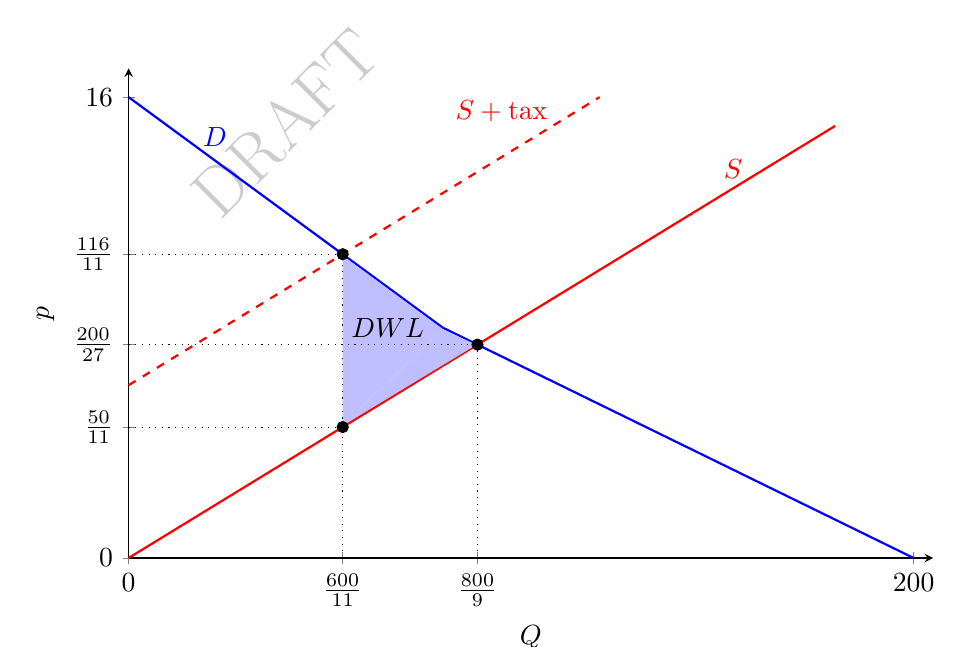
\begin{tikzpicture}
    \begin{axis}[
        width=11.8cm,
        height=7.8cm,
        xmin=0,xmax=205,
        ymin=0,ymax=17,
        axis lines=left,
        xlabel={$Q$},
        ylabel={$p$},
        xtick={0,54.5455,88.8889,200},
        xticklabels={$0$,$\frac{600}{11}$,$\frac{800}{9}$,$200$},
        ytick={0,4.5455,7.4074,10.5455,16},
        yticklabels={$0$,$\frac{50}{11}$,$\frac{200}{27}$,$\frac{116}{11}$,$16$},
        clip=false
    ]
    \addplot[thick,blue] coordinates {(0,16) (80,8)};
    \addplot[thick,blue] coordinates {(80,8) (200,0)};
    \addplot[thick,red,domain=0:180,samples=2] {x/12};
    \addplot[thick,red,dashed,domain=0:120,samples=2] {6 + x/12};

    \addplot[fill=blue!25,draw=none]
        coordinates {(54.5455,4.6) (54.5455,10.5) (80,7.95) (54.5455,4.6)};
    
    \addplot[fill=blue!25,draw=none]
        coordinates {(54.5455,4.6) (80,7.95) (88.6,7.4) (54.5455,4.6)};

    \addplot[dotted] coordinates {(88.8889,0) (88.8889,7.4074)};
    \addplot[dotted] coordinates {(54.5455,0) (54.5455,10.5455)};
    \addplot[dotted] coordinates {(0,10.5455) (54.5455,10.5455)};
    \addplot[dotted] coordinates {(0,4.5455) (54.5455,4.5455)};
    \addplot[dotted] coordinates {(0,7.4074) (88.8889,7.4074)};

    \addplot[only marks,mark=*,mark size=2pt]
        coordinates {(88.8889,7.4074) (54.5455,10.5455) (54.5455,4.5455)};

    \node[blue] at (axis cs:22,14.6) {$D$};
    \node[red] at (axis cs:154,13.5) {$S$};
    \node[red] at (axis cs:95,15.5) {$S+\text{tax}$};
    \node at (axis cs:66,8.0) {$DWL$};
    \end{axis}
    \end{tikzpicture}
    \end{center}
\end{enumerate}

\newpage
\subsubsection{Method 2: Inverse-demand / inverse-supply and welfare geometry}

\begin{enumerate}[label=(\alph*)]
    \item
    The individual demand curves can be written compactly as
    \[
    x_1(p)=\left(2-\frac{p}{8}\right)_+,
    \qquad
    x_2(p)=\left(\frac12-\frac{p}{16}\right)_+,
    \]
    where \((z)_+=\max\{z,0\}\). Equivalently,
    \[
    \boxed{
    x_1(p)=
    \begin{cases}
    2-\dfrac{p}{8}, & 0\le p\le 16,\\
    0, & p>16,
    \end{cases}
    \qquad
    x_2(p)=
    \begin{cases}
    \dfrac12-\dfrac{p}{16}, & 0\le p\le 8,\\
    0, & p>8.
    \end{cases}}
    \]

    \item
    Aggregate demand is
    \[
    Q_D(p)=80\left(2-\frac{p}{8}\right)_+ + 80\left(\frac12-\frac{p}{16}\right)_+.
    \]
    Inverse demand is therefore piecewise:
    \[
    p_D(Q)=
    \begin{cases}
    16-\dfrac{Q}{10}, & 0\le Q\le 80,\\[0.7em]
    \dfrac{200-Q}{15}, & 80\le Q\le 200.
    \end{cases}
    \]
    Hence
    \[
    \boxed{
    p_D(Q)=
    \begin{cases}
    16-\dfrac{Q}{10}, & 0\le Q\le 80,\\[0.7em]
    \dfrac{200-Q}{15}, & 80\le Q\le 200.
    \end{cases}}
    \]

    \item
    Each firm has cost \(3x^2\), so marginal cost is
    \[
    MC(x)=6x.
    \]
    Competitive supply satisfies \(p=MC\), so
    \[
    x_s(p)=\frac{p}{6}.
    \]
    Aggregating across \(n\) firms gives
    \[
    Q_S(p)=\frac{n}{6}p,
    \qquad
    p_S(Q)=\frac{6Q}{n}.
    \]
    Therefore
    \[
    \boxed{Q_S(p)=\frac{n}{6}p,\qquad p_S(Q)=\frac{6Q}{n}.}
    \]

    \item
    Because \(Q_S(p)\) is proportional to \(p\), its elasticity is identically 1:
    \[
    \varepsilon_S=\frac{dQ_S}{dp}\cdot \frac{p}{Q_S}=1.
    \]
    Hence
    \[
    \boxed{\varepsilon_S=1.}
    \]

    \item
    For \(n=72\),
    \[
    p_S(Q)=\frac{Q}{12}.
    \]
    Solve using the lower branch of inverse demand:
    \[
    \frac{200-Q}{15}=\frac{Q}{12}.
    \]
    Therefore
    \[
    12(200-Q)=15Q
    \quad\Longrightarrow\quad
    2400=27Q
    \quad\Longrightarrow\quad
    Q^*=\frac{800}{9}.
    \]
    Then
    \[
    p^*=\frac{Q^*}{12}=\frac{200}{27}.
    \]
    Thus
    \[
    \boxed{Q^*=\frac{800}{9},\qquad p^*=\frac{200}{27}.}
    \]

    \item
    Consumer surplus is the area under inverse demand above price:
    \begin{align*}
    CS
    &=\int_0^{80}\left(16-\frac{Q}{10}\right)\,dQ
      +\int_{80}^{800/9}\left(\frac{200-Q}{15}\right)\,dQ
      -\frac{200}{27}\cdot \frac{800}{9}\\
    &=\frac{89920}{243}.
    \end{align*}
    Producer surplus is
    \[
    PS=\frac12 Q^*p^*
    =\frac12\cdot \frac{800}{9}\cdot \frac{200}{27}
    =\frac{80000}{243}.
    \]
    Hence
    \[
    \boxed{CS=\frac{89920}{243},\qquad PS=\frac{80000}{243}.}
    \]

    \item
    A tax of 6 on producers shifts inverse supply vertically upward by 6:
    \[
    p_{S,t}(Q)=\frac{Q}{12}+6.
    \]
    After tax, the relevant demand branch is the upper one:
    \[
    16-\frac{Q}{10}=\frac{Q}{12}+6.
    \]
    Solving,
    \[
    10=\frac{11Q}{60}
    \quad\Longrightarrow\quad
    Q_t=\frac{600}{11}.
    \]
    Therefore
    \[
    p_b=16-\frac{Q_t}{10}=\frac{116}{11},
    \qquad
    p_s=p_b-6=\frac{50}{11}.
    \]
    The deadweight loss is
    \[
    DWL=\frac12\cdot 6\left(\frac{800}{9}-\frac{600}{11}\right)=\frac{3400}{33}.
    \]
    Thus
    \[
    \boxed{Q_t=\frac{600}{11},\qquad p_b=\frac{116}{11},\qquad p_s=\frac{50}{11},\qquad DWL=\frac{3400}{33}.}
    \]
\end{enumerate}

\newpage
\subsubsection{Method 3: Comparative-statics / elasticity and regime-switch method}

\begin{enumerate}[label=(\alph*)]
    \item
    Write individual demands as
    \[
    x_1(p)=\left(2-\frac{p}{8}\right)_+,
    \qquad
    x_2(p)=\left(\frac12-\frac{p}{16}\right)_+.
    \]
    The cutoffs are therefore
    \[
    p=16 \quad\text{for Type 1,}
    \qquad
    p=8 \quad\text{for Type 2.}
    \]
    So Type 2 exits first as price rises.

    \item
    Aggregate demand is
    \[
    Q_D(p)=80\left(2-\frac{p}{8}\right)_+ + 80\left(\frac12-\frac{p}{16}\right)_+,
    \]
    which gives the two active regimes
    \[
    Q_D(p)=200-15p \quad (0\le p\le 8),
    \qquad
    Q_D(p)=160-10p \quad (8<p\le 16).
    \]
    The structural point is that the demand slope changes when Type 2 exits.

    \item
    Supply is
    \[
    Q_S(p)=\frac{n}{6}p,
    \]
    so changing \(n\) rotates market supply outward through the origin.

    \item
    Even though changing \(n\) changes the level of market supply, the elasticity remains
    \[
    \varepsilon_S=1.
    \]
    Thus
    \[
    \boxed{\text{more firms } \Rightarrow \text{ more supply at each price, but the same elasticity}.}
    \]

    \item
    To determine which demand branch is relevant, compare the supply quantity at \(p=8\):
    \[
    Q_S(8)=\frac{n}{6}\cdot 8=\frac{4n}{3}.
    \]
    If both types are active, then the branch switch occurs at the market kink \((Q,p)=(80,8)\). Hence:
    \[
    \frac{4n}{3} \gtrless 80
    \quad\Longleftrightarrow\quad
    n \gtrless 60.
    \]
    So:
    \begin{itemize}[leftmargin=*]
        \item if \(n>60\), equilibrium lies on the lower branch \(Q_D=200-15p\);
        \item if \(n<60\), equilibrium lies on the upper branch \(Q_D=160-10p\);
        \item if \(n=60\), equilibrium is exactly at the kink.
    \end{itemize}
    Since \(n=72>60\), we use
    \[
    200-15p=12p,
    \]
    which yields
    \[
    \boxed{p^*=\frac{200}{27},\qquad Q^*=\frac{800}{9}.}
    \]

    \item
    Since \(Q^*=\frac{800}{9}>80\), both consumer types remain active in the no-tax equilibrium, but Type 2 buys only a very small amount:
    \[
    x_2^*=\frac{1}{27}.
    \]
    This already suggests that a sufficiently strong tax can push Type 2 completely out of the market.

    Using the area formulas on the aggregate curves,
    \[
    \boxed{CS=\frac{89920}{243},\qquad PS=\frac{80000}{243}.}
    \]

    \item
    After a producer tax \(t=6\), buyer-price supply becomes
    \[
    Q_S^t(p_b)=\frac{n}{6}(p_b-6).
    \]
    For \(n=72\),
    \[
    Q_S^t(p_b)=12p_b-72.
    \]
    Check what happens at the demand cutoff \(p_b=8\):
    \[
    Q_S^t(8)=24,
    \qquad
    Q_D(8)=80.
    \]
    Since taxed supply at \(p_b=8\) is far below demand at the kink, the post-tax equilibrium must occur on the upper branch where only Type 1 remains active. Hence solve
    \[
    160-10p_b=12p_b-72.
    \]
    Therefore
    \[
    \boxed{p_b=\frac{116}{11},\qquad p_s=\frac{50}{11},\qquad Q_t=\frac{600}{11}.}
    \]

    The key comparative-statics insight is that the tax does more than just reduce quantity: it changes the active set of consumers. Type 2 exits completely after tax. The resulting deadweight loss is
    \[
    \boxed{DWL=\frac{3400}{33}.}
    \]
\end{enumerate}

\newpage
\subsubsection{Marking scheme (40 marks)}

\begin{enumerate}[label=(\alph*)]
    \item \textbf{(6 marks)} Individual demand curves
    \begin{itemize}
        \item 2 marks: Correct setup of the Type 1 utility-maximisation problem, including substitution of leftover cash \(m=100-px\) or an equivalent formulation.
        \item 2 marks: Correct derivation of the Type 1 demand curve, including the non-negativity condition.
        \item 2 marks: Correct derivation of the Type 2 demand curve, including the non-negativity condition.
    \end{itemize}

    \item \textbf{(5 marks)} Aggregate demand curve
    \begin{itemize}
        \item 2 marks: Correct identification of the relevant price regions and which consumer types are active in each region.
        \item 2 marks: Correct piecewise aggregation of the two individual demand curves.
        \item 1 mark: Correct final aggregate demand curve, including the kink / cutoff structure.
    \end{itemize}

    \item \textbf{(5 marks)} Individual and aggregate supply
    \begin{itemize}
        \item 2 marks: Correct setup of the firm’s profit-maximisation problem.
        \item 1 mark: Correct individual supply curve.
        \item 2 marks: Correct aggregate supply curve for \(n\) identical firms.
    \end{itemize}

    \item \textbf{(4 marks)} Market elasticity of supply
    \begin{itemize}
        \item 2 marks: Correct elasticity result, including whether it changes with the number of firms.
        \item 2 marks: Clear economic explanation of why the elasticity does or does not change as \(n\) varies.
    \end{itemize}

    \item \textbf{(7 marks)} Equilibrium for \(n=72\)
    \begin{itemize}
        \item 2 marks: Correct substitution of \(n=72\) into the aggregate supply curve.
        \item 2 marks: Correct identification of the relevant branch of aggregate demand.
        \item 2 marks: Correct equilibrium price and quantity.
        \item 1 mark: Diagram with demand, supply, and the exact equilibrium correctly indicated.
    \end{itemize}

    \item \textbf{(5 marks)} Consumer and producer surplus
    \begin{itemize}
        \item 2 marks: Correct computation of consumer surplus.
        \item 2 marks: Correct computation of producer surplus.
        \item 1 mark: Correct final expressions / values, consistent with the equilibrium from part (e).
    \end{itemize}

    \item \textbf{(8 marks)} Per-unit tax on producers
    \begin{itemize}
        \item 2 marks: Correct setup of the post-tax equilibrium, including the tax wedge between buyers’ and sellers’ prices.
        \item 2 marks: Correct taxed prices and quantity, or a fully correct equivalent derivation.
        \item 2 marks: Correct deadweight welfare loss, or a correct DWL triangle with correct dimensions.
        \item 2 marks: Diagram and explanation correctly showing the incidence of the tax burden on consumers and producers.
    \end{itemize}
\end{enumerate}

%====================================================
% Sample Question 2
%====================================================
\newpage
\section{Sample Question 2: Teddy Bears}

\subsection{Problem}

\noindent
Consider the market for teddy bears. \footnote{There appears to be a likely typo in the handout. If the individual supply curve is written as \(S(p)=4p-100\), then positive supply requires \(p\ge 25\), while market demand \(D(p)=1000-80p\) falls to zero at \(p=12.5\). Hence there is no interior trade equilibrium, so the later tax and deadweight-loss parts become degenerate. The intended version is very likely \(S(p)=4p-10\), which yields a standard non-degenerate competitive-equilibrium and welfare-analysis problem.} There are \(n\) firms with \emph{individual} supply curves given by
\[
S(p)=4p-10.
\]
The \emph{market} demand curve is given by
\[
D(p)=1000-80p.
\]

\begin{enumerate}[label=(\alph*)]
    \item Derive the market supply curve in terms of \(n\). \hfill \textbf{(5 marks)}
    \item Suppose there is a per-unit tax of \$5 on the \emph{consumers}. For \(n=10\), draw out the market supply and demand curves \emph{with} and \emph{without} tax, indicating and explaining the deadweight welfare loss from the tax. \hfill \textbf{(9 marks)}
    \item For the same per-unit tax on consumers, calculate the deadweight welfare loss as a function of the number of producers in the market \(n\). \hfill \textbf{(10 marks)}
    \item How does the deadweight welfare loss change with the number of producers? Explain the intuition behind this. \hfill \textbf{(6 marks)}
\end{enumerate}

\newpage
\subsection{Solution}

\subsubsection{Method 1: Direct aggregation and tax-wedge algebra}

\begin{enumerate}[label=(\alph*)]
    \item
    Each firm supplies
    \[
    q_i(p)=4p-10.
    \]
    With \(n\) identical firms, market supply is
    \[
    Q_S(p)=n(4p-10)=4np-10n.
    \]
    Therefore
    \[
    \boxed{Q_S(p)=4np-10n.}
    \]

    \item
    For \(n=10\), the market supply curve is
    \[
    Q_S(p)=40p-100.
    \]
    Demand is
    \[
    Q_D(p)=1000-80p.
    \]

    Before tax, equilibrium satisfies
    \[
    1000-80p=40p-100.
    \]
    Hence
    \[
    1100=120p
    \quad\Longrightarrow\quad
    p^*=\frac{55}{6}.
    \]
    Then
    \[
    Q^*=1000-80p^*
    =1000-80\cdot \frac{55}{6}
    =\frac{800}{3}.
    \]

    Thus
    \[
    \boxed{p^*=\frac{55}{6},\qquad Q^*=\frac{800}{3}.}
    \]

    Now impose a per-unit tax of 5 on consumers. Let \(p_b\) be the buyers' price and \(p_s\) the sellers' price. Then
    \[
    p_b=p_s+5.
    \]
    Demand is
    \[
    Q_D=1000-80p_b,
    \]
    while supply depends on the sellers' price:
    \[
    Q_S=40p_s-100.
    \]
    Substitute \(p_s=p_b-5\):
    \[
    Q_S=40(p_b-5)-100=40p_b-300.
    \]
    Equate demand and supply:
    \[
    1000-80p_b=40p_b-300.
    \]
    Hence
    \[
    1300=120p_b
    \quad\Longrightarrow\quad
    p_b=\frac{65}{6}.
    \]
    Therefore
    \[
    p_s=p_b-5=\frac{35}{6}.
    \]
    The taxed quantity is
    \[
    Q_t=1000-80p_b
    =1000-80\cdot \frac{65}{6}
    =\frac{400}{3}.
    \]

    Thus
    \[
    \boxed{p_b=\frac{65}{6},\qquad p_s=\frac{35}{6},\qquad Q_t=\frac{400}{3}.}
    \]

    The deadweight loss is
    \(
    DWL=\frac12\cdot 5\left(\frac{800}{3}-\frac{400}{3}\right)=\frac{1000}{3}.
    \)
    Hence $\quad \boxed{DWL=\frac{1000}{3}.}$

    A suitable graph\footnote{Although the solution represents the consumer tax as an upward shift of supply, an equivalent and often clearer representation is a downward shift of demand, which more directly reflects the tax being levied on consumers. Both approaches impose the same wedge \(p_b - p_s = t\) and yield identical equilibrium outcomes.} is:

    \begin{center}
    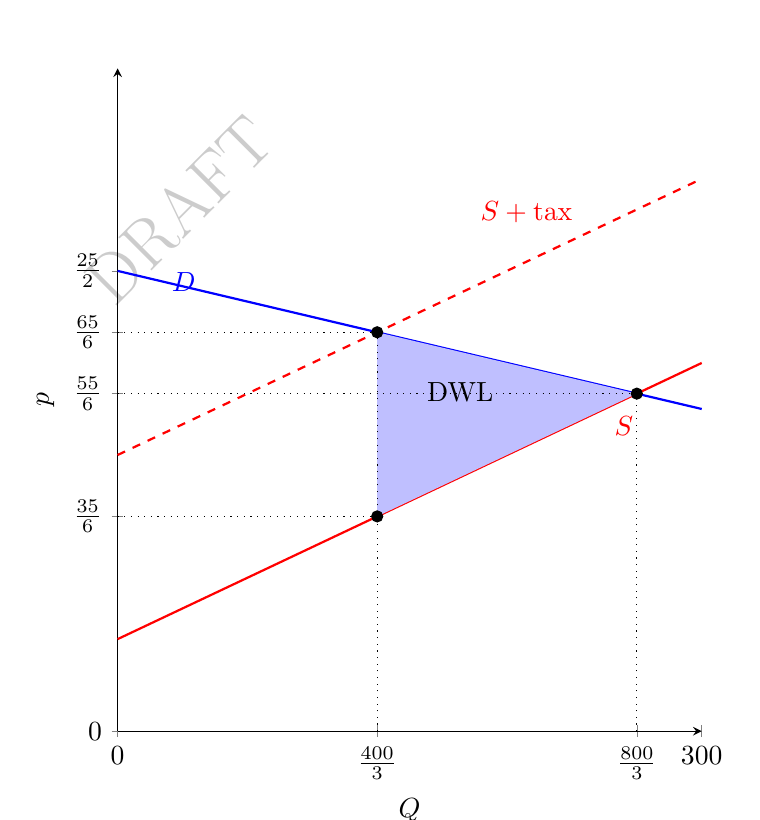
\begin{tikzpicture}
    \begin{axis}[
        width=9cm,
        height=10cm,
        xmin=0,xmax=300,
        ymin=0,ymax=18,
        axis lines=left,
        xlabel={$Q$},
        ylabel={$p$},
        xtick={0,133.3333,266.6667,300},
        xticklabels={$0$,$\frac{400}{3}$,$\frac{800}{3}$,$300$},
        ytick={0,5.8333,9.1667,10.8333,12.5},
        yticklabels={$0$,$\frac{35}{6}$,$\frac{55}{6}$,$\frac{65}{6}$,$\frac{25}{2}$},
        clip=false
    ]
    \addplot[thick,blue,domain=0:300,samples=2] {12.5 - x/80};
    \addplot[thick,red,domain=0:300,samples=2] {2.5 + x/40};
    \addplot[thick,red,dashed,domain=0:300,samples=2] {7.5 + x/40};

    \addplot[fill=blue!25,draw=none]
        coordinates {(133.3333,5.8333) (133.3333,10.8333) (266.6667,9.1667) (133.3333,5.8333)};

    \addplot[dotted] coordinates {(266.6667,0) (266.6667,9.1667)};
    \addplot[dotted] coordinates {(133.3333,0) (133.3333,10.8333)};
    \addplot[dotted] coordinates {(0,9.1667) (266.6667,9.1667)};
    \addplot[dotted] coordinates {(0,10.8333) (133.3333,10.8333)};
    \addplot[dotted] coordinates {(0,5.8333) (133.3333,5.8333)};

    \addplot[only marks,mark=*,mark size=2pt]
        coordinates {(266.6667,9.1667) (133.3333,10.8333) (133.3333,5.8333)};

    \node[blue] at (axis cs:34,12.2) {$D$};
    \node[red] at (axis cs:260,8.3) {$S$};
    \node[red] at (axis cs:210,14.1) {$S+\text{tax}$};
    \node at (axis cs:176,9.2) {DWL};
    \end{axis}
    \end{tikzpicture}
    \end{center}

    \item
    For general \(n\), before tax:
    \[
    1000-80p=4np-10n.
    \]
    So
    \[
    1000+10n=(80+4n)p
    \quad\Longrightarrow\quad
    p^*(n)=\frac{1000+10n}{80+4n}.
    \]
    The corresponding quantity is
    \[
    Q_0(n)=1000-80p^*(n)=\frac{800n}{n+20}.
    \]

    After a consumer tax of 5:
    \[
    p_b=p_s+5.
    \]
    Since
    \[
    Q_S=4np_s-10n,
    \]
    in terms of the buyers' price we have
    \[
    Q_S=4n(p_b-5)-10n=4np_b-30n.
    \]
    Equating with demand:
    \[
    1000-80p_b=4np_b-30n.
    \]
    Therefore
    \[
    1000+30n=(80+4n)p_b,
    \]
    and the taxed quantity is
    \[
    Q_t(n)=1000-80p_b=\frac{400n}{n+20}.
    \]

    Thus
    \[
    DWL(n)=\frac12\cdot 5\bigl(Q_0(n)-Q_t(n)\bigr)
    =\frac12\cdot 5\left(\frac{800n}{n+20}-\frac{400n}{n+20}\right).
    \]
    Hence
    \[
    \boxed{DWL(n)=\frac{1000n}{n+20}.}
    \]

    \item
    Since
    \[
    DWL(n)=\frac{1000n}{n+20},
    \]
    we differentiate:
    \[
    \frac{d}{dn}DWL(n)=\frac{20000}{(n+20)^2}>0.
    \]
    Therefore deadweight loss increases with the number of producers. Moreover,
    \[
    \lim_{n\to\infty}DWL(n)=1000.
    \]
    So
    \[
    \boxed{\text{DWL increases with }n\text{ and tends to }1000\text{ as }n\to\infty.}
    \]

    Intuitively, more firms make aggregate supply more elastic, so a given tax causes a larger quantity distortion and therefore a larger deadweight loss.
\end{enumerate}

\newpage
\subsubsection{Method 2: Inverse-demand / inverse-supply and welfare geometry}

\begin{enumerate}[label=(\alph*)]
    \item
    Since
    \[
    Q_S=4np-10n,
    \]
    the inverse supply curve is
    \[
    p_S(Q)=\frac{Q+10n}{4n}=\frac{Q}{4n}+\frac52.
    \]
    Thus
    \[
    \boxed{Q_S(p)=4np-10n,\qquad p_S(Q)=\frac{Q}{4n}+\frac52.}
    \]

    \item
    Inverse demand is
    \[
    p_D(Q)=\frac{1000-Q}{80}=\frac{25}{2}-\frac{Q}{80}.
    \]
    For \(n=10\), inverse supply is
    \[
    p_S(Q)=\frac{Q}{40}+\frac52.
    \]
    Before tax:
    \[
    \frac{25}{2}-\frac{Q}{80}=\frac{Q}{40}+\frac52.
    \]
    Thus
    \[
    10=\frac{3Q}{80}
    \quad\Longrightarrow\quad
    Q^*=\frac{800}{3}.
    \]
    Then
    \[
    p^*=\frac{25}{2}-\frac{1}{80}\cdot \frac{800}{3}=\frac{55}{6}.
    \]

    With a consumer tax of 5, the buyers' supply curve shifts up by 5:
    \[
    p_{S,t}(Q)=\frac{Q}{40}+\frac{15}{2}.
    \]
    Equating with inverse demand:
    \[
    \frac{25}{2}-\frac{Q}{80}=\frac{Q}{40}+\frac{15}{2}.
    \]
    Therefore
    \[
    5=\frac{3Q}{80}
    \quad\Longrightarrow\quad
    Q_t=\frac{400}{3}.
    \]
    The buyers' price is
    \[
    p_b=\frac{25}{2}-\frac{1}{80}\cdot \frac{400}{3}=\frac{65}{6},
    \]
    and the sellers' price is
    \[
    p_s=p_b-5=\frac{35}{6}.
    \]

    Hence
    \[
    \boxed{Q^*=\frac{800}{3},\quad p^*=\frac{55}{6},\quad Q_t=\frac{400}{3},\quad p_b=\frac{65}{6},\quad p_s=\frac{35}{6}.}
    \]

    The deadweight loss is
    \[
    DWL=\frac12\cdot 5\left(\frac{800}{3}-\frac{400}{3}\right)=\frac{1000}{3}.
    \]
    Therefore
    \[
    \boxed{DWL=\frac{1000}{3}.}
    \]

    \item
    For general \(n\), inverse supply is
    \[
    p_S(Q)=\frac{Q}{4n}+\frac52,
    \]
    while inverse demand is
    \[
    p_D(Q)=\frac{25}{2}-\frac{Q}{80}.
    \]

    Before tax:
    \[
    \frac{25}{2}-\frac{Q}{80}=\frac{Q}{4n}+\frac52.
    \]
    Hence
    \[
    10=Q\left(\frac{1}{80}+\frac{1}{4n}\right)
    =Q\frac{n+20}{80n},
    \]
    so
    \[
    Q_0(n)=\frac{800n}{n+20}.
    \]

    With tax \(t=5\), buyer-side inverse supply is
    \[
    p_{S,t}(Q)=\frac{Q}{4n}+\frac{15}{2}.
    \]
    Therefore
    \[
    \frac{25}{2}-\frac{Q}{80}=\frac{Q}{4n}+\frac{15}{2}
    \quad\Longrightarrow\quad
    5=Q\frac{n+20}{80n},
    \]
    so
    \[
    Q_t(n)=\frac{400n}{n+20}.
    \]
    Hence
    \[
    DWL(n)=\frac12\cdot 5\left(Q_0(n)-Q_t(n)\right)
    =\frac12\cdot 5\cdot \frac{400n}{n+20}
    =\frac{1000n}{n+20}.
    \]
    Therefore
    \[
    \boxed{DWL(n)=\frac{1000n}{n+20}.}
    \]

    \item
    Since the inverse supply slope is
    \[
    \frac{dp_S}{dQ}=\frac{1}{4n},
    \]
    it becomes flatter as \(n\) rises. Thus supply becomes more elastic, the tax causes a larger reduction in quantity, and deadweight loss rises. Therefore
    \[
    \boxed{\text{More producers } \Rightarrow \text{ more elastic supply } \Rightarrow \text{ larger DWL}.}
    \]
\end{enumerate}

\newpage
\subsubsection{Method 3: Concise olympiad-style tax-parameter method}

\begin{enumerate}[label=(\alph*)]
    \item
    Market supply is
    \[
    \boxed{Q_S(p)=4np-10n.}
    \]
    Equivalently,
    \[
    \boxed{p_S(Q)=\frac{Q}{4n}+\frac52.}
    \]

    \item
    For \(n=10\), inverse demand and supply are
    \[
    p_D(Q)=\frac{25}{2}-\frac{Q}{80},
    \qquad
    p_S(Q)=\frac{Q}{40}+\frac52.
    \]
    Introduce a general consumer tax \(t\). Then buyer-side inverse supply becomes
    \[
    p_{S,t}(Q)=\frac{Q}{40}+\frac52+t.
    \]
    Equilibrium is defined by
    \[
    \frac{25}{2}-\frac{Q}{80}=\frac{Q}{40}+\frac52+t.
    \]
    Rearranging,
    \[
    10-t=\frac{3Q}{80}.
    \]
    So
    \[
    Q_t=\frac{80}{3}(10-t).
    \]
    Therefore:
    \[
    Q_0=\frac{80}{3}(10)=\frac{800}{3},
    \qquad
    Q_5=\frac{80}{3}(5)=\frac{400}{3}.
    \]
    Then
    \[
    p^*=\frac{25}{2}-\frac{1}{80}\cdot \frac{800}{3}=\frac{55}{6},
    \]
    \[
    p_b=\frac{25}{2}-\frac{1}{80}\cdot \frac{400}{3}=\frac{65}{6},
    \qquad
    p_s=p_b-5=\frac{35}{6}.
    \]
    Therefore
    \[
    \boxed{p^*=\frac{55}{6},\quad Q^*=\frac{800}{3},\quad p_b=\frac{65}{6},\quad p_s=\frac{35}{6},\quad Q_t=\frac{400}{3}.}
    \]
    The deadweight loss follows immediately:
    \[
    DWL=\frac12\cdot 5\left(\frac{800}{3}-\frac{400}{3}\right)=\frac{1000}{3}.
    \]
    Hence
    \[
    \boxed{DWL=\frac{1000}{3}.}
    \]

    \item
    For general \(n\), buyer-side inverse supply with tax \(t\) is
    \[
    p_{S,t}(Q)=\frac{Q}{4n}+\frac52+t.
    \]
    Equilibrium solves
    \[
    \frac{25}{2}-\frac{Q}{80}=\frac{Q}{4n}+\frac52+t.
    \]
    Hence
    \[
    10-t=Q\left(\frac{1}{80}+\frac{1}{4n}\right)
    =Q\frac{n+20}{80n}.
    \]
    So the equilibrium quantity under tax \(t\) is
    \[
    \boxed{Q_t(n)=\frac{80n(10-t)}{n+20}.}
    \]
    In particular,
    \[
    Q_0(n)=\frac{800n}{n+20},
    \qquad
    Q_5(n)=\frac{400n}{n+20}.
    \]
    Therefore
    \[
    DWL(n)=\frac12\cdot 5\left(Q_0(n)-Q_5(n)\right)
    =\frac12\cdot 5\cdot \frac{400n}{n+20}.
    \]
    Thus
    \[
    \boxed{DWL(n)=\frac{1000n}{n+20}.}
    \]

    \item
    The formula
    \[
    DWL(n)=\frac{1000n}{n+20}
    \]
    is increasing in \(n\), because
    \[
    \frac{d}{dn}DWL(n)=\frac{20000}{(n+20)^2}>0.
    \]
    So
    \[
    \boxed{\text{DWL increases with }n.}
    \]
    This method is structurally concise because one solves the whole tax family at once via the parameter \(t\), then specialises to \(t=0\) and \(t=5\).
\end{enumerate}

\newpage
\subsubsection{Marking scheme (30 marks)}

\begin{enumerate}[label=(\alph*)]
    \item \textbf{(5 marks)} Market supply curve
    \begin{itemize}
        \item 2 marks: Correct aggregation of the individual supply curves across \(n\) firms.
        \item 2 marks: Correct simplified market supply curve in terms of \(n\).
        \item 1 mark: Correct treatment of the economically relevant domain / interpretation of the supply curve.
    \end{itemize}

    \item \textbf{(9 marks)} Tax analysis for \(n=10\)
    \begin{itemize}
        \item 2 marks: Correct market supply curve for \(n=10\).
        \item 2 marks: Correct no-tax equilibrium analysis and/or correct identification of the no-tax market outcome.
        \item 2 marks: Correct treatment of the consumer tax wedge and post-tax equilibrium analysis.
        \item 2 marks: Correct deadweight welfare loss conclusion, including a correct explanation.
        \item 1 mark: Diagram clearly showing the relevant demand and supply curves, with and without tax, together with the relevant equilibrium information.
    \end{itemize}

    \item \textbf{(10 marks)} Deadweight welfare loss as a function of \(n\)
    \begin{itemize}
        \item 3 marks: Correct no-tax equilibrium analysis in terms of \(n\), or a correct general argument about the pre-tax market outcome.
        \item 3 marks: Correct post-tax equilibrium analysis in terms of \(n\), or a correct general argument about the post-tax market outcome.
        \item 3 marks: Correct derivation of deadweight welfare loss as a function of \(n\).
        \item 1 mark: Correct final simplified expression.
    \end{itemize}

    \item \textbf{(6 marks)} Comparative statics of deadweight welfare loss
    \begin{itemize}
        \item 2 marks: Correct statement of how deadweight welfare loss changes with the number of producers.
        \item 2 marks: Correct supporting reasoning using the shape / elasticity / position of market supply.
        \item 2 marks: Clear economic intuition connecting the number of producers to the quantity distortion and welfare loss.
    \end{itemize}
\end{enumerate}
\end{document}
